\documentclass{article}

\PassOptionsToPackage{numbers,compress}{natbib}
\usepackage[sglblindworkshop]{neurips_2026}
\workshoptitle{Machine Learning for Systems (MLForSys)}

\usepackage[utf8]{inputenc}
\usepackage[T1]{fontenc}
\usepackage{booktabs}
\usepackage{microtype}
\usepackage{xcolor}
\usepackage{hyperref}
\usepackage{url}
\usepackage{graphicx}
\usepackage{float}

\definecolor{ftblue}{HTML}{2F75B5}
\definecolor{ftlight}{HTML}{EAF2F8}
\newcommand{\system}{\textsc{FreeToken-MLX}}
\newcommand{\code}[1]{\texttt{#1}}

\title{FreeToken-MLX: Memory-Bounded MoE Inference on Apple Silicon}

\author{Anonymous Author(s)}

\begin{document}
\maketitle

\begin{abstract}
MoE models activate few parameters per token but retain an expert pool that can
exceed edge-device memory. We present \system, an Apple Silicon backend inside
FreeToken that preserves its cross-layer expert bank, cache, eviction, and
offload path while executing selected experts with MLX. It chooses resident MLX
when safe and bounded offload otherwise, and can quantize only routed experts.
On one 16GB Apple M4, stock BF16 MLX failed before token one; bounded BF16
offload generated at 1.88 token/s. Expert-only Q4 reached 4.49 token/s at
7.93GB peak. Under an equal cache-byte budget, Q3 gate/up and Q4 down improved
128-token throughput by 11.1\% over uniform Q4. This single-device study shows
a memory--throughput Pareto path, not universal superiority over resident MLX.
\end{abstract}

\section{Motivation and contribution}

Sparse activation reduces arithmetic but not expert storage. Prior systems page
experts on personal devices~\citep{xue2024moeinfinity,eliseev2023offloading,yi2023edgemoe};
FreeToken instead builds a shared elastic cache and adapts execution to hardware
bandwidth~\citep{yang2026freetoken}. Its release primarily targets CUDA.
Apple Silicon instead exposes unified CPU/GPU memory through MLX
\citep{hannun2023mlx}; eagerly materializing a large checkpoint can still
exceed the safe working set and terminate inference or displace other
applications.

\system adapts FreeToken rather than building an independent engine. It
contributes: (1) an MLX backend reusing the expert bank, global cache, counters,
and eviction; (2) safe resident/offload selection with explicit headroom; and
(3) routed-expert-only, projection-aware precision. The scope is batch-one
Qwen1.5-MoE-A2.7B on Apple Silicon.

\section{System design}

\begin{figure}[H]
  \centering
  \setlength{\fboxsep}{4pt}
  \small
  \colorbox{ftlight}{\parbox{0.20\linewidth}{\centering Dense/router/\\shared BF16}}
  $\rightarrow$
  \colorbox{ftlight}{\parbox{0.13\linewidth}{\centering top-$k$\\routing}}
  $\rightarrow$
  \colorbox{ftlight}{\parbox{0.20\linewidth}{\centering selected-expert\\MLX compute}}\\[5pt]
  \fbox{\parbox{0.18\linewidth}{\centering safetensor\\expert bank}}
  $\rightarrow$
  \colorbox{ftlight}{\parbox{0.22\linewidth}{\centering bounded global\\LRU / SLRU cache}}
  $\nearrow$
  \caption{Only router-selected experts enter the MLX compute graph;
  FreeToken's expert bank and bounded cache remain on the serving path.}
  \label{fig:design}
\end{figure}

\paragraph{Execution and caching.}
Dense attention, router, and shared-expert tensors remain resident MLX arrays.
Routed tensors remain separate safetensors entries addressed by
$(\mathrm{layer},\mathrm{expert})$. The router synchronizes only its small
top-$k$ index tensor. Each selection performs a FreeToken cache lookup: a hit
reuses evaluated MLX arrays; a miss materializes the expert bank entry and may
evict a previous expert. Periodic graph evaluation bounds lazy references that
would otherwise keep evicted weights alive. Logs expose real hits, misses, and
evictions.

\paragraph{Memory safety and hybrid selection.}
The runtime estimates resident peak memory from checkpoint, packing, runtime,
and optional draft-model bytes. It selects resident MLX only within both the
MLX limit and physical memory minus requested headroom under current pressure.
Otherwise it budgets the expert cache after dense/runtime reserves. If one
expert cannot fit, startup fails; cache shrinkage is monotonic per request.

\paragraph{Expert precision.}
The converter streams BF16 shards, preserves non-routed weights, and applies
MLX affine packing only to routed projections. Uniform Q4 is default; opt-in Q3
gate/up with Q4 down reduces routed-expert storage about 16.7\%, admitting more
experts per byte. This is a layout integration, not a new quantizer;
mixed-precision offloading has precedent~\citep{tang2024hobbit}.

\section{Evaluation}

We evaluate Qwen1.5-MoE-A2.7B~\citep{qwen2024moe} (24 layers, 60 routed
experts/layer, top-4), batch one, on an Apple M4 with 16GB unified memory,
macOS 15.3, Python 3.12.13, and MLX-LM 0.31.3. Generation is greedy from
\code{Hello}. Safety-sensitive runs cap MLX at 10GB and reserve 3.2GB of system
headroom. Peaks are MLX allocator measurements rather than total macOS memory.
The first three rows in Table~\ref{tab:results} use different token counts and
show deployment feasibility; the final two form the controlled comparison.

\begin{figure}[H]
  \centering
  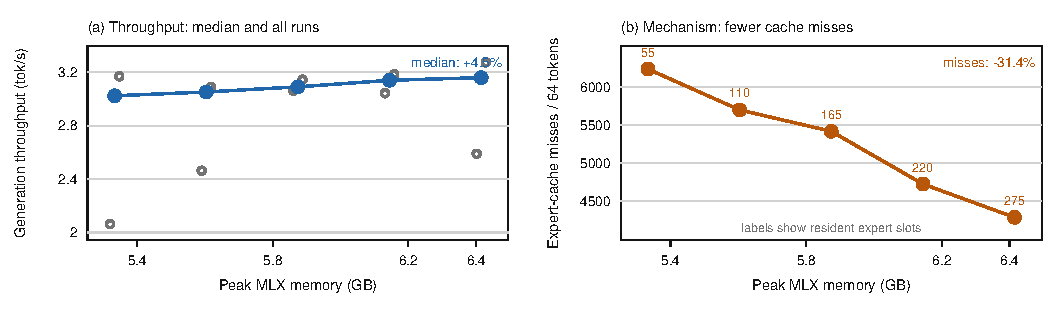
\includegraphics[width=0.90\linewidth]{figures/memory_throughput_curve.pdf}
  \caption{Q4 cache sweep (64 tokens, $n=3$ fresh processes/point, 45s cooldown,
  rotating order): all throughput observations and medians; misses are labelled
  by slots. Moving 55--275 slots raised peak 5.33--6.42GB, cut misses 31.4\%,
  and raised median throughput 4.5\%; overlapping ranges limit the claim.}
  \label{fig:memory-curve}
\end{figure}

\begin{table}[t]
\centering
\caption{Measured feasibility and equal-budget precision ablation. $^*$Peak
reported by MLX before Metal OOM.}
\label{tab:results}
\scriptsize
\setlength{\tabcolsep}{3.2pt}
\begin{tabular}{lrrrrr}
\toprule
Path & Tokens & Slots & Misses & tok/s & Peak \\
\midrule
Stock MLX-LM BF16 & 0 & -- & -- & -- & 28.63GB$^*$ \\
FreeToken BF16 offload & 32 & 121 & -- & 1.88 & 5.83GB \\
BF16 dense / Q4 experts & 32 & 864 & -- & 4.49 & 7.93GB \\
Uniform Q4 experts & 128 & 864 & 3,489 & 7.31 & 8.02GB \\
Q3 gate/up, Q4 down & 128 & 1,015 & 2,822 & 8.12 & 8.03GB \\
\bottomrule
\end{tabular}
\end{table}

\paragraph{Capacity and throughput.}
Stock \code{mlx-lm} attempted to materialize BF16, reported 28.63GB, and failed
before token one. Bounded FreeToken offload completed 32 tokens at 1.88 token/s
and 5.83GB. This path adds capacity, but expert reads remain the main bottleneck.
Quantizing routed experts alone reached 4.49 token/s at 7.93GB, $2.39\times$ the
reported BF16-offload rate while retaining dense, attention, router, and shared
weights in BF16. It changes routed-expert numerics and is therefore a separate
Pareto point, not a lossless speedup.

\paragraph{Controlled projection ablation.}
With fixed pressure, a 10GB limit, 3.2GB headroom, prompt, and cache bytes, we
interleaved two fresh runs per layout. Projection-aware precision admitted
1,015 rather than 864 experts, cut misses 19.1\%, and reduced paired mean time
from 17.52s to 15.77s (7.31 to 8.12 token/s, +11.1\%) at nearly equal peak.
Forced to 864 slots, it remained 3.4\% faster and used 0.62GB less peak memory.

\paragraph{Quality proxy and negative evidence.}
A 135-token proxy yielded NLL 2.618 (BF16), 2.707 (Q4), 2.725 (Q3/Q3/Q4), and
2.865 (Q3). It cannot establish quality, so Q4 remains default; expert stacking
and a grouped-Q4 kernel both slowed end-to-end execution.

\bibliographystyle{plainnat}
\bibliography{references}

\end{document}
